
%(BEGIN_QUESTION)
% Copyright 2006, Tony R. Kuphaldt, released under the Creative Commons Attribution License (v 1.0)
% This means you may do almost anything with this work of mine, so long as you give me proper credit

Examine the following electronic level switch circuit:

$$\includegraphics[width=15.5cm]{i00513x01.eps}$$

Identify what kinds of process liquids this level switch would be applicable to, and why.  Also, identify which ladder-logic switch symbol would be appropriate for this particular level switch:

$$\includegraphics[width=15.5cm]{i00513x02.eps}$$

Qualitatively determine the following component voltage drops in the circuit with low level and with high level (i.e. write ``low'' or ``high'' voltage rather than try to calculate actual values):

% No blank lines allowed between lines of an \halign structure!
% I use comments (%) instead, so that TeX doesn't choke.

$$\vbox{\offinterlineskip
\halign{\strut
\vrule \quad\hfil # \ \hfil & 
\vrule \quad\hfil # \ \hfil & 
\vrule \quad\hfil # \ \hfil \vrule \cr
\noalign{\hrule}
%
% First row
{\bf Component} & {\bf Low-level condition} & {\bf High-level condition} \cr
%
\noalign{\hrule}
%
% Another row
$R1$ &  &  \cr
%
\noalign{\hrule}
%
% Another row
$Q1$ (between drain and source) &  &  \cr
%
\noalign{\hrule}
%
% Another row
Relay coil &  &  \cr
%
\noalign{\hrule}
} % End of \halign 
}$$ % End of \vbox


\vfil 

\underbar{file i00513}
\eject
%(END_QUESTION)





%(BEGIN_ANSWER)

This is a graded question -- no answers or hints given!

%(END_ANSWER)





%(BEGIN_NOTES)

An important fact to recall regarding MOSFET transistors is that this is an E-type (enhancement-type) MOSFET, and as such is normally-off.  Being an {\it N-channel} MOSFET, a {\it positive} gate signal is required to turn it on.  Specifically, the applied gate voltage must be of such a polarity that the gate is more positive than the transistor substrate.  This will turn the MOSFET on and allow current to go through to the relay coil to energize it and close the switch contacts.

\vskip 10pt

A resistor connecting the MOSFET's gate terminal to the +15 volt power supply rail provides the necessary bias to turn the transistor on when no liquid touches the probe.  This energizes the relay and closes the switch contacts, so that the contacts are closed when the probe is dry.  This, by definition, is a {\it normally-closed} liquid level switch.

\vskip 10pt

When liquid level rises up high enough to contact the probe, it shorts the probe to ground.  This forces the MOSFET gate to a zero-volt condition, causing the MOSFET to return to its natural (off) state.  This de-energizes the relay, causing its switch contacts to open.  Thus, a high-level condition causes the switch contacts to open: the behavior we would expect from a {\bf normally-closed} liquid level switch.

\vskip 10pt

Obviously, this switch only functions on {\it conductive} liquids.

% No blank lines allowed between lines of an \halign structure!
% I use comments (%) instead, so that TeX doesn't choke.

$$\vbox{\offinterlineskip
\halign{\strut
\vrule \quad\hfil # \ \hfil & 
\vrule \quad\hfil # \ \hfil & 
\vrule \quad\hfil # \ \hfil \vrule \cr
\noalign{\hrule}
%
% First row
{\bf Component} & {\bf Low-level condition} & {\bf High-level condition} \cr
%
\noalign{\hrule}
%
% Another row
$R1$ & low & high \cr
%
\noalign{\hrule}
%
% Another row
$Q1$ (between drain and source) & low & high \cr
%
\noalign{\hrule}
%
% Another row
Relay coil & high & low \cr
%
\noalign{\hrule}
} % End of \halign 
}$$ % End of \vbox

\vskip 10pt

An interesting detail to note in this circuit is the {\it commutating diode} connected in parallel with the relay coil.  Note how its orientation ensures an ``off'' (non-conducting) state while the relay coil is energized.  The sole purpose of this diode is to provide a non-destructive path for current through the coil as its magnetic field collapses (imemdiately after its has been turned off) and the polarity across the coil reverses (acting as a source of electrical energy now rather than as a load).

%INDEX% Switch, level: liquid conductivity

%(END_NOTES)


